\section{The comparison morphism} \label{Section comparison morphism}
In this appendix we recall the construction of the comparison morphism for $\PP^N$ and how it can be used to show that the stable map and the quasimap invariants of projective space coincide. This has been proven in \cite[Theorem 3]{MOP} and \cite[Section 4.3]{Manolache-Push} (but see also \cite[Proposition 4.1]{Bertram} and \cite[Theorem 7.1]{Popa-Roth} for inspiration).

\subsection{Construction of the comparison morphism}
In order to give a morphism $\chi\colon\M{g}{n}{\PP^N}{d}\to\Q{g}{n}{\PP^N}{d}$ we need to be able to associate, to a family of stable maps on a base $B$, a family of quasimaps on the same base.

The pointwise construction is as follows: any stable map defines a quasimap with no basepoints. The only thing that might prevent this quasimap from being stable is the presence of rational tails (of positive degree, by the stability condition for stable maps). Let $C=C^{(0)}\sqcup_{q_i}R_i$ be the source curve; there is a ``permanent'' subcurve $C^{(0)}$ which is joined to a number of rational tails $R_i$ each of which has degree $d_i>0$. We let $q_i$ be the node connecting $C^{(0)}$ and $R_i$; note that it is the only special point of $R_i$, and hence all the marked points belong to $C^{(0)}$. We obtain a stable quasimap by collapsing the rational tails and introducing basepoints of length $d_i$ at each of the (former) nodes $q_i$.

In other words, the comparison map is given by sending the quasimap $((C,x_1,\ldots,x_n),L,u_0,\ldots,u_N))$ to 
\begin{equation*}((C^{(0)},x_1,\ldots,x_n),L|_{C^{(0)}}(\Sigma_i d_i q_i),\hat{u}_0,\ldots,\hat{u}_N) \end{equation*}
where $\hat{u}_i$ is obtained from $u_i|_{C^{(0)}}$ via the natural inclusion:
\begin{equation*} L|_{C^{(0)}}\to L|_{C^{(0)}}(\Sigma_i d_i q_i) \end{equation*}
Locally around $q_j$ this has the effect of multiplying each $u_i$ by the $d_j$th power of the equation defining $q_j$, thus introducing a basepoint of length $d_j$.

The construction in families requires us to find a line bundle on the universal curve that is trivial on the rational tails (which we wish to contract) and relatively ample elsewhere. This can be performed at the level of Picard stacks: let $\mathfrak{Pic}_{g,n}^{d,\text{st}}$ be the open substack of $\mathfrak{Pic}(\pi\colon\mathfrak{C}_{g,n}\to\mathfrak{M}_{g,n})$ obtained by requiring that the total degree of the line bundle is $d$, the degree on each component is nonnegative and $\mathcal L\otimes\omega_{\pi}(\Sigma_i x_i)$ is ample relative to $\pi$, where $\mathcal L$ is the universal line bundle.

Let $T^{\delta}$ be the locus in the universal curve $\mathfrak{C}_{\mathfrak{Pic}}$ over $\mathfrak{Pic}_{g,n}^{d,\text{st}}$ consisting of rational tails on which $\mathcal L$ has degree $\delta$; since the stack $\mathfrak{C}_{\mathfrak{Pic}}$ is smooth, $T^{\delta}$ is a Cartier divisor. Notice that $T^{\delta_0}$ and $T^{\delta_1}$ (say with $\delta_0<\delta_1$) intersect in a stratum of codimension $1$, where the rational tail splits into two rational components, the furthest from $C^{(0)}$ having degree $\delta_0$:

\begin{center}
\begin{tikzpicture}
 \draw[help lines] (-1,-1) grid (1,1);
 \node[below] at (0,-1) {$T^{\delta_0}$};
 \node[right] at (1,0) {$T^{\delta_1}$};
 
 \draw[gray] (0,-.5) -- (-2,0);
 \draw[decorate,decoration={snake,amplitude=2pt}] (-4,0) -- (-2.5,0);
 \draw (-3.8,-.2) -- node[left]{$\delta_0$} (-3.8,1.3);
 
 \draw[gray] (0,0) -- (-.5,1.5);
 \draw[-,decorate,decoration={snake,amplitude=2pt}] (-1,2) -- (.5,2);
 \draw (-.8,1.8) -- node[left]{$\delta_1-\delta_0$} (-.8,3.3);
 \draw (-1,3) -- node[above]{$\delta_0$} (0.5,3.5);
 
 \draw[gray] (.5,0) -- (2,.5);
 \draw[decorate,decoration={snake,amplitude=2pt}] (2.5,.5) -- (4,.5);
 \draw (2.7,.3) -- node[left]{$\delta_1$} (2.7,1.8);
 
\draw[fill=black] (0,0) circle [radius=1.5pt];
 \draw[fill=black] (0,-.5) circle [radius=1.5pt];
 \draw[fill=black] (.5,0) circle [radius=1.5pt];
 \end{tikzpicture}
\end{center}
\medskip

Define the following line bundle on $\mathfrak{C}_{\mathfrak{Pic}}$:
\begin{equation*} \mathcal N=\mathcal L\otimes\omega_{\pi}(\Sigma_i x_i)\otimes\bigotimes_{0<\delta\leq d}\mathcal O_{\mathfrak{C}_{\mathfrak{Pic}}}((\delta-1) T^\delta) \end{equation*}
We claim that $\mathcal{N}$ is trivial on every component of every rational tail, and $\pi$-relatively ample elsewhere. Consider a curve $C^{(0)}\sqcup_q R$ with a rational tail of degree $e$. We first consider the simple case where $R$ is isomorphic to a chain of $\PP^1$s. We label the components $R^{(1)},\ldots,R^{(n)}$, numbered from the closest to the farthest from $C^{(0)}$. We let $e_i$ denote the degree of $R^{(i)}$. We set $T_i=\bigcup_{j=i}^n R_j$ and $\epsilon_i=\deg \mathcal{L}|_{T_i} - 1 = e-1-\sum_{j=1}^{i-1} e_j$. The picture is as follows:

\begin{center}
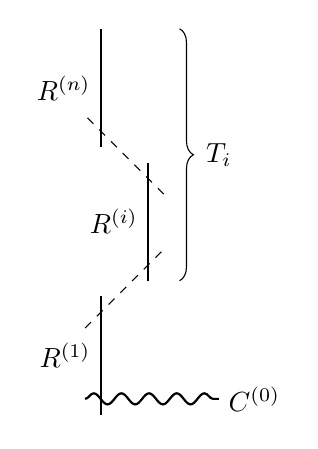
\begin{tikzpicture}
  \draw[thick,decorate,decoration={snake,amplitude=2pt}] (-.2,.2) -- (1.5,.2);
  \node[right] at (1.5,.2) {$C^{(0)}$};
  \draw[thick] (0,0) -- node[left]{$R^{(1)}$} (0,1.5);
  \draw[dashed] (-.2,1.1) -- (.8,2.1);
  \draw[thick] (.6,1.7) -- node[left]{$R^{(i)}$} (.6,3.2);
  \draw[dashed] (.8,2.8) -- (-.2,3.8);
  \draw[thick] (0,3.4) -- node[left]{$R^{(n)}$} (0,4.9);
  \draw [decorate,decoration={brace,amplitude=5pt,mirror}] (1,1.7) -- (1,4.9) node [midway,xshift=.5cm]{$T_i$};
 \end{tikzpicture}
\end{center}

The local structure of $\mathfrak{Pic}_{g,n}^{d,\text{st}}$ means that a general one-parameter family inside this stack will give us a smoothing of our curve. The total space of such a family is a normal surface $S$; thus we can compute the degree of the restriction of $\mathcal{N}$ to the irreducible components of the central fiber of this family by first restricting $\mathcal{N}$ to $S$, and then using intersection theory on the normal surface $S$.

Notice first that $T^\delta|_S = T_{i_\delta}$ where $i_\delta$ is the unique value of $i$ such that
\begin{equation*} \delta = \sum_{j=i_{\delta}}^n e_i \end{equation*}
and if no such $i_\delta$ exists then $T^\delta|_S = 0$. Thus we obtain:
\begin{equation*} \bigotimes_{0<\delta\leq d}\mathcal{O}_{\mathfrak{C}_{\mathfrak{Pic}}}((\delta-1) T^\delta)|_S = \mathcal{O}_S(\Sigma_{j=1}^n \epsilon_j T_j) \end{equation*}
Now, $R^{(i)}$ has self-intersection $-2$ for $i=1,\ldots,n-1$, and so we have
\begin{equation*}
R^{(i)}\cdot T_j =
  \begin{cases}
    0 & \text{for } j<i \\
    -1 & \text{for } j=i \\
    1 & \text{for } j=i+1 \\
    0 & \text{for } j>i+1
  \end{cases}
\end{equation*}
from which it follows that:
\begin{equation*} \deg \mathcal{N}|_{R^{(i)}} = \deg \mathcal{L}|_{R^{(i)}} - \epsilon_i + \epsilon_{i+1} = e_i - e_i = 0 \end{equation*}
On the other hand $R^{(n)}$ has self-intersection $-1$ and so we have
\begin{equation*}
R^{(n)} \cdot T_j =
\begin{cases}
0 & \text{for } j < n \\
-1 & \text{for } j = n
\end{cases}
\end{equation*}
which implies:
\begin{equation*} \deg \mathcal{N}|_{R^{(n)}} = \deg \mathcal{L}|_{R^{(n)}} - 1 - \epsilon_n = e_n - 1 - (e_n-1) = 0\end{equation*}
Here we have used the fact that $\omega_\pi(\Sigma_i x_i)$ has degree $0$ on $R^{(i)}$ for $i=1,\ldots,n-1$ and has degree $-1$ on $R^{(n)}$. Thus $\mathcal{N}$ is trivial on every component on every rational tail, as claimed. The fact that it is $\pi$-relatively ample on the rest of the curve follows from the stability condition and the fact that $\OO_{\mathfrak{C}_{\mathfrak{Pic}}}(T^\delta)$ is effective when restricted to $C^{(0)}$.

In the above discussion we restricted ourselves to the simple case where $R$ is a chain of $\PP^1$s. In general, however, $R$ can be an arbitrary tree of $\PP^1$s. The argument in this case is similar, though combinatorially more complex. For brevity we will discuss one example:

\begin{center}
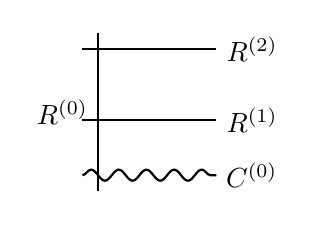
\begin{tikzpicture}
  \draw[thick,decorate,decoration={snake,amplitude=2pt}] (-.2,.2) -- (1.5,.2);
  \node[right] at (1.5,.2) {$C^{(0)}$};
  \draw[thick] (0,0) -- node[left]{$R^{(0)}$} (0,2);
  \draw[thick] (-.2,.9) -- (1.5,.9) node[right]{$R^{(1)}$};
  \draw[thick] (-.2,1.8) -- (1.5,1.8) node[right]{$R^{(2)}$};
\end{tikzpicture}
\end{center}

Here $R$ has $3$ irreducible components $R^{(0)},R^{(1)},R^{(2)}$ with degrees $e_0,e_1,e_2$ respectively. Let $e = e_0+e_1+e_2$ be the total degree of the rational tail.

Of the divisors $T^{\delta}$ for $0<\delta\leq d$, the total space $S$ only intersects\footnote{Notice in particular that $S$ does not intersect $T^{e_0}$ or $T^{e_0+e_1}$ (unless $e_0=0$).} $T^{e_1}, T^{e_2}$ and $T^e$. We have:
\begin{align*}
T^{e_1}|_S & = R^{(1)} \\
T^{e_2}|_S & = R^{(2)} \\
T^e|_S & = R = R^{(0)} + R^{(1)} + R^{(2)}
\end{align*}
Let us first look at $R^{(1)}$. This has self-intersection $-1$ and so:
\begin{equation*} R^{(1)} \cdot T^{e_1}|_S = -1 \qquad R^{(1)} \cdot T^{e_2}|_S = 0 \qquad R^{(1)} \cdot T^e|_S = 1-1 = 0 \end{equation*}
Thus we obtain
\begin{equation*} \deg \mathcal{N}|_{R^{(1)}} = \deg \mathcal{L}|_{R^{(1)}} - 1 - (e_1 - 1) = 0 \end{equation*}
and same argument applies to $R^{(2)}$. On the other hand, $R^{(0)}$ has self-intersection $-3$ (in general, a component that appears with $n$ adjacent components will have self-intersection $-n$). We have
\begin{equation*} R^{(0)} \cdot T^{e_1}|_S = 1 \qquad R^{(0)} \cdot T^{e_2}|_S = 1 \qquad R^{(0)} \cdot T^e|_S = -3 + 1 + 1 = -1 \end{equation*}
and thus we obtain
\begin{align*} \deg \mathcal{N}|_{R^{(0)}} & = \deg \mathcal{L}|_{R^{(0)}} + 1 + (e_1 - 1) + (e_2 - 1) - (e-1) \\
& = e_0 + e_1 + e_2 - e = 0 \end{align*}
as required.

To summarise, then: we have constructed a line bundle $\mathcal{N}$ on $\mathfrak{C}_{\mathfrak{Pic}}$ which is trivial on the components that we wish to contract and $\pi$-relatively ample elsewhere. By taking the relative Proj construction we therefore obtain another curve
\begin{equation*} \hat{\mathfrak{C}}_{\mathfrak{Pic}}:=\underline{\operatorname{Proj}}_{\mathfrak{Pic}_{g,n}^{d,\operatorname{st}}} \left(\bigoplus_{k\geq 0}\pi_*\mathcal{N}^{\otimes k}\right) \end{equation*}
over $\mathfrak{Pic}_{g,n}^{d,\text{st}}$, and a map $\sst$ which contracts the rational tails
\bcd
\mathfrak C_{\mathfrak{Pic}}\ar[r,"\sst"]\ar[dr,"\pi" left=3pt] & \hat{\mathfrak{C}}_{\mathfrak{Pic}} \ar[d,"\hat{\pi}"]\\
 & \mathfrak{Pic}_{g,n}^{d,\text{st}}
\ecd
The map $\hat{\pi}$ is flat since it is a family of genus $g$ curves over a reduced base. Furthermore, it can be checked using cohomology and base-change \cite[Theorem 12.11]{HAR} \cite[Corollary 1.5]{Knudsen} (notice that the fibers of $\sst$ are either points or rational curves) that
\begin{equation*}\hat{\mathcal L}:=\sst_*\left(\mathcal L\otimes \bigotimes_{0<\delta\leq d}\mathcal{O}_{\hat{\mathfrak{C}}_{\mathfrak{Pic}}}(\delta T^\delta)\right) \end{equation*}
is a line bundle on $\hat{\mathfrak{C}}_{\mathfrak{Pic}}$ of degree $d$ relative to $\hat{\pi}$. By the Yoneda lemma we thus obtain a comparison morphism $\tilde{\comp}$ fitting into a commutative diagram:
\bcd
\mathfrak C_{\mathfrak{Pic}}\ar[r,"\sst"]\ar[dr,"\pi" left=3pt] & \hat{\mathfrak{C}}_{\mathfrak{Pic}} \ar[d,"\hat{\pi}"]\ar[dr,phantom,"\square" right=-0.5pt]\ar[r] & \mathfrak C_{\mathfrak{Pic}}\ar[d,"\pi"] \\
 & \mathfrak{Pic}_{g,n}^{d,\text{st}}\ar[r,"\tilde{\comp}"] & \mathfrak{Pic}_{g,n}^{d,\text{st}}
\ecd
This discussion all took place at the level of Picard stacks. If we work instead at the level of stable maps and quasimaps the same arguments apply to construct the contracted curve $\hat{\mathcal{C}}_{\mathcal{M}}$ and line bundle $\hat{\mathcal{L}}$. Furthermore we can push down the sections $u_i$ from $\mathcal{C}_{\mathcal{M}}$ to $\hat{\mathcal{C}}_{\mathcal{M}}$ because they are constant on the contracted rational tails (notice that they automatically acquire basepoints). This gives rise to a comparison morphism:
\begin{equation*} \comp\colon \M{g}{n}{\PP^N}{d}\to\Q{g}{n}{\PP^N}{d} \end{equation*}
We have a commutative diagram
\bcd
\M{g}{n}{\PP^N}{d} \ar[d,"\nu_{\mathcal{N}}"]\ar[r,"\comp"] & \Q{g}{n}{\PP^N}{d}\ar[d,"\nu_{\mathcal Q}"] \\
\mathfrak{Pic}_{g,n}^{d,\text{st}}\ar[r,"\tilde{\comp}"] & \mathfrak{Pic}_{g,n}^{d,\text{st}}
\ecd
and, as before, a diagram of universal curves:
\bcd
\mathcal C_{\mathcal{M}}\ar[r,"\sst"] \ar[rd,"\pi_{\mathcal{N}}" left=3pt] & \hat{\mathcal{C}}_{\mathcal{M}}=\comp^*\mathcal C_{\mathcal Q} \ar[d,"\hat{\pi}_{\mathcal{N}}"]\ar[dr,phantom,"\square"]\ar[r] & \mathcal C_{\mathcal Q}\ar[d,"\pi_{\mathcal Q}"] \\
 & \M{g}{n}{\PP^N}{d}\ar[r,"\comp"] & \Q{g}{n}{\PP^N}{d}
\ecd

\subsection{The comparison morphism preserves the virtual classes}
For $\PP^N$ the stable map and quasimap invariants coincide; we have:
\begin{equation*} \comp_* \virt{\M{g}{n}{\PP^N}{d}} = \virt{\Q{g}{n}{\PP^N}{d}} \end{equation*}
The proof of this fact, following \cite{Manolache-Push}, rests on the construction of a relative perfect obstruction theory
\begin{equation*} \mathbf{E}_{\comp} \to \mathbf{L}_{\comp} \end{equation*}
for the morphism $\comp$. The construction is best outlined in the arXiv version of \cite[Remark 5.20]{Manolache-Push}. Let $\tilde{\nu}_{\mathcal{N}}$ denote the composition:
\bcd
\M{g}{n}{\PP^N}{d} \ar[r,"\nu_{\mathcal{N}}"] \ar[rr,"{\tilde{\nu}}_{\mathcal{N}}", bend right=25pt] & \mathfrak{Pic}_{g,n}^{d,\operatorname{st}} \ar[r,"\tilde{\comp}"] & \mathfrak{Pic}_{g,n}^{d,\operatorname{st}}
\ecd
We may endow this morphism with a relative perfect obstruction theory via the following morphism of exact triangles:
\bcd
\nu_\mathcal{N}^*\mathbf L_{\tilde{\comp}}\ar[d]\ar[r] & \mathbf E_{\tilde{\nu}_{\mathcal{N}}} \ar[d]\ar[r] & \mathbf E_{\nu_\mathcal{N}} \ar[d]\ar[r,"{[1]}"] & {}\\
\nu_\mathcal{N}^*\mathbf L_{\tilde{\comp}}\ar[r] & \mathbf L_{\tilde{\nu}_{\mathcal{N}}} \ar[r] & \mathbf L_{\nu_\mathcal{N}} \ar[r,"{[1]}"] & {}
\ecd
Notice that $\tilde{\comp}$ is a morphism between smooth Artin stacks. As such we can examine the exact triangle of cotangent complexes induced by $\tilde{\comp}$ and conclude that $\mathbf{L}_{\tilde{\comp}}$ is supported in $[-1,1]$. It then follows easily  that $\mathbf E_{\tilde{\nu}_{\mathcal{N}}}$ is also supported in $[-1,1]$; in order to show that it is perfect, we consider the long exact cohomology sequence near $\h^1(\mathbf E_{\tilde{\nu}_{\mathcal{N}}})$:
\begin{equation*} \h^{0}(\mathbf E_{\nu_\mathcal{N}}) \to \h^{1}(\nu_\mathcal{N}^*\mathbf L_{\tilde{\comp}}) \to \h^{1} (\mathbf E_{\tilde{\nu}_{\mathcal{N}}}) \to 0 \end{equation*}
We must show that the morphism $\h^0 (\mathbf{E}_{\nu_{\mathcal{N}}}) \to \h^1(\nu_{\mathcal{N}}^* \mathbf{L}_{\tilde{\comp}})$ is surjective. Looking at the dual picture, we see that the map
\begin{equation*} \h^{1}(\nu_\mathcal{N}^*\mathbf{L}_{\tilde{\comp}})^\vee \to \h^{0}(\mathbf E_{\nu_\mathcal{N}})^\vee \cong \h^{0}(\mathbf{L}_{\nu_\mathcal{N}})^\vee \end{equation*}
is injective, because every infinitesimal automorphism of the rational tail induces a nontrivial deformation of the stable map, since the degree of the stable map is positive on every component of the rational tail. We conclude that $\h^{1}\mathbf E_{\tilde{\nu}_{\mathcal{N}}}=0$ and so indeed $\mathbf{E}_{\tilde{\nu}_{\mathcal{N}}}$ is a perfect obstruction theory for $\tilde{\nu}_{\mathcal{N}}$. It induces the usual virtual fundamental class on the moduli space of stable maps.

Now, we can construct a morphism of obstruction theories (see 
\cite[Lemma 4.19]{Manolache-Push})
\begin{equation*} \comp^*\mathbf E_{\nu_\mathcal Q}\to\mathbf E_{\nu_\mathcal{N}} \end{equation*}
as follows. We have
\begin{align*} \mathbf E^\vee_{\nu_\mathcal{N}}& =\R\pi_{\mathcal{N}*}\mathcal L^{\oplus N+1}=\R\hat\pi_* \sst_*\mathcal L^{\oplus N+1} \\
\comp^*\mathbf E^\vee_{\nu_\mathcal Q} & = \chi^* \R \pi_{\mathcal{Q}} \hat{\mathcal{L}}^{\oplus{N+1}} = \R {\hat{\pi}}_{\mathcal{N}*}\hat{\mathcal L}^{\oplus N+1}\end{align*}
where $\hat{\mathcal L}=\sst_*\left(\mathcal L\otimes \bigotimes_{0<\delta\leq d}\mathcal O_{\mathfrak C}(\delta T^\delta)\right)$. Thus $\mathbf E^\vee_{\nu_\mathcal{N}}\to\comp^*\mathbf E^\vee_{\nu_\mathcal Q}$ comes from the following inclusion of line bundles on $\mathcal C_\mathcal{N}$:
\[
\mathcal L\hookrightarrow \mathcal L\otimes \bigotimes_{0<\delta\leq d}\mathcal O_{\mathfrak C}(\delta T^\delta).
\]
We now claim that this morphism factors through $\mathbf E_{\tilde{\nu}_{\mathcal{N}}}$. Examining the diagram:
\bcd
& \comp^*\mathbf E_{\nu_\mathcal Q}\ar[dl,dashed,"\exists ?"]\ar[d]\ar[dr,"\phi"] & \\
\mathbf E_{\tilde{\nu}_{\mathcal{N}}} \ar[r] & \mathbf E_{\nu_\mathcal{N}}\ar[r] & \nu_\mathcal{N}^*\mathbf L_{\tilde{\comp}}[1] \ar[r,"{[1]}"] & \,
\ecd
we see that it is equivalent to show that $\phi$ is the zero map. This follows formally from the factorisation:
\bcd
 & & \mathbf L_\comp \ar[ld,"{[1]}" swap] & & \\
\comp^* \mathbf E_{\nu_\mathcal Q}\ar[dd]\ar[r] & \comp^*\mathbf L_{\nu_\mathcal Q}\ar[rr] &  & \mathbf L_{\tilde{\nu}_{\mathcal{N}}}\ar[ul]\ar[dd] & \\
 & & & & \nu_{\mathcal{N}}^*\mathbf L_{\tilde{\comp}}[1]\ar[ul,"{[1]}" swap] \\
\mathbf E_{\nu_\mathcal{N}} \ar[rrr] & & & \mathbf L_{\nu_\mathcal{N}}\ar[ur] & {}
\ecd
We thus obtain a morphism
\begin{equation*} \psi \colon \comp^* \mathbf{E}_{\nu_{\mathcal{Q}}} \to \mathbf{E}_{\tilde{\nu}_{\mathcal{N}}} \end{equation*}
and the cone $C(\psi)$ gives a relative obstruction theory for the comparison morphism $\chi$. A priori, it is supported in $[-2,0]$. By the octahedral axiom we have:
%-------------
\begin{comment}
\begin{center}
\begin{tikzcd}[execute at end picture={
    \begin{scope}[on background layer]
    \fill[pattern=north east lines, pattern color=gray!20] (a.north west) -- (b.north east) -- (b.south east) -- (a.south west) -- cycle;
    \fill[pattern=north west lines, pattern color=gray!20] (c.north west) -- (c.north east) -- (d.south east) -- (d.south west) -- cycle;
    \end{scope}
  }]
\comp^* \mathbb E_{\nu_\mathcal Q}\ar[d]\ar[r] & |[alias=a]| \comp^*\mathbb L_{\nu_\mathcal Q}\ar[r] & |[alias=c]|\mathbb L_{\tilde{\nu}_{\mathcal{N}}}\ar[r]\ar[d] & |[alias=b]| \mathbb L_\comp \\
\mathbb E_{\nu_\mathcal{N}} \ar[rr] & & \mathbb L_{\nu_\mathcal{N}}\ar[d] & \\
 & & |[alias=d]| \nu_{\mathcal{N}}^*\mathbb L_{\comp '}[1]
\end{tikzcd}
\end{center} 
\end{comment}
\begin{comment}
Dually, we look at $\nu_\mathcal{N}^*\mathbb T_{\tilde{\comp}}[-1]\xrightarrow{\phi^\vee} \R\hat\pi_*(\hat{\mathcal L}^{\oplus r+1})$. Notation: call $R$ the rational tail, joined at the rest of the curve (which we denote by $(C^{(0)},\mathbf p)$ as a marked curve), at the node $q$, which we may occasionally think of as a (smooth) point on $C^{(0)}$. We claim that:
\begin{itemize}
 \item $h^0(\phi^\vee)$ is zero because: the LHS involves automorphisms of the rational tail that leave $C^{(0)}$ fixed, while the RHS involves deformations of $C^{(0)}$, so there is no possible interference.
 \item $h^1(\phi^\vee)$ is zero because: \textcolor{red}{this is slightly awkward.} There are two types of possible contributions to the LHS. They correspond to either moving the node $q$ along $C^{(0)}$, or smoothing it. The former appears in the relative tangent of $\chi'$ only if the marked curve $(C^{(0)},\mathbf p)$ has no automorphisms that may ``move $q$ back'', i.e. $(C^{(0)},\mathbf p)$ is a stable pointed curve. The latter matters only if $(C^{(0)},q,\mathbf p)$ has no moduli, i.e. $(C^{(0)},\mathbf p)$ is a rational tail with less than 3 markings. \textcolor{red}{I will try to justify why the first type vanishes under $h^1(\phi^\vee)$, and leave the second type because I do not understand it as yet.} Look at the long exact sequence
\begin{align*}
  0 &\to \Hom(\Omega_{C^{(0)}},\mathcal O_{C^{(0)}}(-q-\sum p_i)) &\to \Hom(\Omega_{C^{(0)}},\mathcal O_{C^{(0)}}(-\sum p_i)) &\to \\
  T_{C^{(0)},q} &\to \Ext^1(\Omega_{C^{(0)}},\mathcal O_{C^{(0)}}(-q-\sum p_i)) &\to \Ext^1(\Omega_{C^{(0)}},\mathcal O_{C^{(0)}}(-\sum p_i)) &\to 0
 \end{align*}
We are interested in what happens to
\[
 \frac{T_{C^{(0)},q}}{\operatorname{Im}\left( \Hom(\Omega_{C^{(0)}},\mathcal O_{C^{(0)}}(-\sum p_i)) \right)}
\]
under $h^1(\phi^\vee)$. If we can show that $h^1(\phi^\vee)$ factors through $\Ext^1(\Omega_{C^{(0)}},\mathcal O_{C^{(0)}}(-\sum p_i))$ we are in business. Indeed the natural maps
\bcd
\Def_L\ar[d]\ar[r] & \Def_{(C,L)}\ar[d]\ar[r] & \Def_C\ar[d] \\
H^1(\mathcal O_C)\ar[r] & H^1(L^{\oplus r+1})\ar[r] & H^1(f^*T_{\PP^N})
\ecd
show that $h^1(\phi^\vee)$ factors through
\[
\Ext^1(\Omega_{C^{(0)}},\mathcal O_{C^{(0)}}(-q-\sum p_i))\to \Ext^1(\Omega_{C^{(0)}},\mathcal O_{C^{(0)}})\to \Ext^1(f^*\Omega_{\PP^N},\mathcal O_{C^{(0)}})\simeq H^1(f^*T_{\PP^N}).
\]
 \item $h^2(\phi^\vee)$ is zero because: $\mathbb E^\vee_{\tilde{\nu}_{\mathcal{N}}}$ is supported in $[0,1]$.
\end{itemize}
\end{comment}
%----------------------
\begin{center}
 \begin{tikzcd}[cramped]
  \comp^*\mathbf E_{\nu_\mathcal{Q}} \ar[dd,"\psi"]\ar[rrdd,"\tilde{\psi}"] & & & & & & \\
& & & & & & \\
\mathbf E_{\tilde{\nu}_\mathcal{N}}\ar[dd]\ar[rr] & & \mathbf E_{\nu_\mathcal{N}} \ar[rrrr]\ar[dr] & & & & \nu_{\mathcal{N}}^*\mathbf L_{\tilde{\comp}}{[1]} \\
& & & C(\tilde{\psi})\ar[urrr] & & & \\
C(\psi) \ar[urrr] & & & & & & 
 \end{tikzcd}
\end{center}
Now $C(\psi)$ is supported in $[-1,0]$ \cite[Lemma 4.20]{Manolache-Push} and $\nu_{\mathcal{N}}^*\mathbf L_{\tilde{\comp}}{[1]}$ is supported in degrees $[-2,0]$, from which it follows that $C(\psi)=\mathbf E_{\comp}$ is a perfect obstruction theory. The conclusion, that
\begin{equation*} \comp_*\virt{\M{g}{n}{\PP^N}{d}}=\virt{\Q{g}{n}{\PP^N}{d}} \end{equation*}
follows from the connectedness of $\M{g}{n}{\PP^N}{d}$ \cite{KP}, hence of $\Q{g}{n}{\PP^N}{d}$, and an application of the virtual push-forward theorem \cite[Proposition 4.21]{Manolache-Push}.

\subsection{An example where the comparison morphism fails to exist}
We will now explain with an example the reason why a naive attempt to extend the comparison morphism to a general toric variety fails. The problem boils down to the fact that not all toric divisors are nef: a rational tail contained in a such divisor may have a corresponding line bundle with negative degree $-d$; when contracting such a rational tail, we take the line bundle $L|_{C^{(0)}}(-dq)$, but it is not clear what to do with the sections. We would like to divide them by $z^d$, where $z$ is a local coordinate around $q$, but we are by no means guaranteed that this is possible. Put differently, we now have an inclusion $L|_{C^{(0)}}(-dq)\hookrightarrow L|_{C^{(0)}}$, but the given sections of $L$ do not necessarily live in the image of $H^0(C^{(0)},L|_{C^{(0)}}(-dq))\to H^0(C^{(0)},L|_{C^{(0)}})$.

A concrete example can be found by looking at the Hirzebruch surface $\mathbb F_1=\operatorname{Bl}_{p}\PP^2$. Since we may choose the point $p$ to be a torus-fixed point of $\PP^2$, $\mathbb{F}_1$ is a toric variety; see Figures \ref{Figure toric fan}, \ref{Figure nef cone} and \ref{Figure Mori cone}.
\begin{figure}[h]
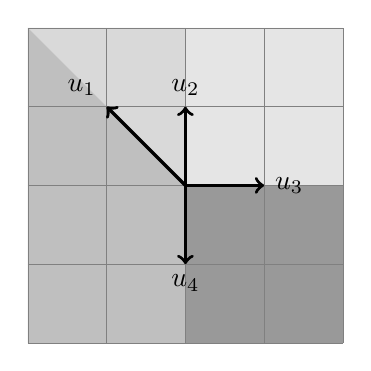
\begin{tikzpicture}
\path [fill=black!10!white] (0,0) -- (2,0) -- (2,2) -- (0,2) -- (0,0);
\path [fill=black!15!white] (0,0) -- (-2,2) -- (0,2) -- (0,0);
\path [fill=black!25!white] (0,0) -- (-2,2) -- (-2,-2) -- (0,-2) -- (0,0);
\path [fill=black!40!white] (0,0) -- (0,-2) -- (2,-2) -- (2,0) -- (0,0);
\draw [help lines] (-2,-2) grid (2,2);
\draw [->,very thick] (0,0) -- (-1,1) node[above left]{$u_1$};
\draw [->,very thick] (0,0) -- (0,1) node[above]{$u_2$};
\draw [->,very thick] (0,0) -- (1,0) node[right]{$u_3$};
\draw [->,very thick] (0,0) -- (0,-1) node[below]{$u_4$};
\end{tikzpicture}
\caption{Toric fan for $\mathbb F_1$.}
\label{Figure toric fan}
\end{figure}
\begin{figure}
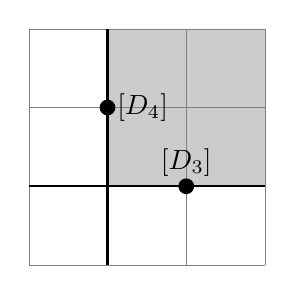
\begin{tikzpicture}
\path [fill=black!20!white] (0,0) -- (2,0) -- (2,2) -- (0,2) -- (0,0);
\draw [help lines] (-1,-1) grid (2,2);
\fill [black] (0,1) circle[radius=.1] node[right]{${[D_4]}$};
\fill [black] (1,0) circle[radius=.1] node[above]{${[D_3]}$};
\draw [thick] (-1,0) -- (2,0);
\draw [thick] (0,-1) -- (0,2);
\end{tikzpicture}
\caption{Nef cone $\operatorname{Nef}(\mathbb F_1)$.}
\label{Figure nef cone}
\end{figure}
\begin{figure}
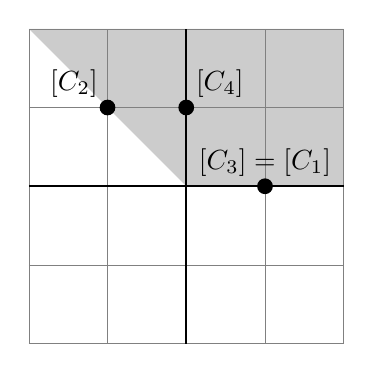
\begin{tikzpicture}
\path [fill=black!20!white] (0,0) -- (2,0) -- (2,2) -- (-2,2) -- (0,0);
\draw [help lines] (-2,-2) grid (2,2);
\fill [black] (0,1) circle[radius=.1] node[above right]{${[C_4]}$};
\fill [black] (1,0) circle[radius=.1] node[above]{${[C_3]}={[C_1]}$};
\fill [black] (-1,1) circle[radius=.1] node[above left]{${[C_2]}$};
\draw [thick] (-2,0) -- (2,0);
\draw [thick] (0,-2) -- (0,2);
\end{tikzpicture}
\caption{Mori cone $\overline{\operatorname{NE}}(\mathbb F_1)$.}
\label{Figure Mori cone}
\end{figure}

The group $\Pic(\mathbb F_1)$ is generated by $[D_3]$ and $[D_4]$, with relations $[D_1]=[D_3]$ and $[D_2]=[D_4]-[D_3]$; the intersection form is given by:
\[
{}
\begin{cases}
 [D_3]^2=0 \\
 [D_3]\cdot [D_4]=1 \\
 [D_4]^2=1
\end{cases} 
\]
When we are thinking of the $D_i$ as curves instead of as divisors, we will denote them by $C_i$. The space $\mathbb F_1$ can be viewed as a $\PP^1$-bundle over $\PP^1$, in which case $C_1$ and $C_3$ represent the fibers of the bundle (over the torus-fixed points of $\PP^1$), while $C_4$ and $C_2$ are the zero and infinity sections, respectively. When thinking of $\mathbb F_1$ as $\operatorname{Bl}_{p}\PP^2$, $C_2$ is the exceptional divisor, $C_4$ is the toric line not passing through $p$, and $C_1,C_3$ are the strict transforms of the toric lines through $p$.

Let us examine the moduli space $\M{0}{2}{\mathbb F_1}{[C_2]+[C_4]}$. Since $[C_4] = [C_2]+[C_3]$ we have $[C_2]+[C_4] = 2[C_2] + [C_3]$. We can thus consider the locus of stable maps inside this moduli space such that:
\begin{enumerate}
\item the source curve splits up as $C=R_1 \sqcup_q R_2$, with all of the marked points belonging to $R_1$;
\item $R_1$ is mapped isomorphically to a fibre (hence $f_*[R_1] = [C_3]$);
\item $R_2$ is a degree-$2$ covering of $C_2 \cong \PP^1$ (hence $f_*[R_2]=2[C_2]$).
\end{enumerate}
The component $R_2$ is a rational tail and so should be contracted by the comparison morphism. However, the line bundle $L_2$ on $C$ corresponding to the divisor $D_2$ has degree $-2$ when restricted to $R_2$ (the degree is equal to $[D_2] \cdot f_*[R_2]=2[D_2]^2 = -2$). Thus when we contract $R_2$ we should replace $L_2|_{R_1}$ by $L_2|_{R_1}(-2q)$. However, the section $u_2|_{R_1}$ only comes from a section of $L_2|_{R_1}(-2q)$ if it vanishes to order $2$ at $q$, that is, $q$ is a ramification point for the degree $2$ cover. This is certainly not the case in general. Thus we see that in this example the comparison morphism does not exist.

\begin{comment}

\textcolor{blue}{Something is going on here: in this case there is a boundary component where the map is of the type that we have just described, and the requirement that $u_{2|R_1}$ vanishes of order $2$ at the node defines precisely the intersection with the main component. Check this. Could we possibly exploit this phenomenon to define a smaller compactification, possibly even smaller than quasimaps?} 

\end{comment}